% !TEX TS-program = pdflatex
% !TEX encoding = UTF-8 Unicode

% This is a simple template for a LaTeX document using the "article" class.
% See "book", "report", "letter" for other types of document.

\documentclass[11pt]{article} % use larger type; default would be 10pt

\usepackage[utf8]{inputenc} % set input encoding (not needed with XeLaTeX)

%%% Examples of Article customizations
% These packages are optional, depending whether you want the features they provide.
% See the LaTeX Companion or other references for full information.

%%% PAGE DIMENSIONS
\usepackage{geometry} % to change the page dimensions
\geometry{a4paper} % or letterpaper (US) or a5paper or....
% \geometry{margin=2in} % for example, change the margins to 2 inches all round
% \geometry{landscape} % set up the page for landscape
%   read geometry.pdf for detailed page layout information

\usepackage{graphicx} % support the \includegraphics command and options

% \usepackage[parfill]{parskip} % Activate to begin paragraphs with an empty line rather than an indent

%%% PACKAGES
\usepackage{booktabs} % for much better looking tables
\usepackage{array} % for better arrays (eg matrices) in maths
\usepackage{paralist} % very flexible & customisable lists (eg. enumerate/itemize, etc.)
\usepackage{verbatim} % adds environment for commenting out blocks of text & for better verbatim
\usepackage{subfig} % make it possible to include more than one captioned figure/table in a single float
% These packages are all incorporated in the memoir class to one degree or another...

%%% HEADERS & FOOTERS
\usepackage{fancyhdr} % This should be set AFTER setting up the page geometry
\pagestyle{fancy} % options: empty , plain , fancy
\renewcommand{\headrulewidth}{0pt} % customise the layout...
\lhead{}\chead{}\rhead{}
\lfoot{}\cfoot{\thepage}\rfoot{}

%%% SECTION TITLE APPEARANCE
\usepackage{sectsty}
\allsectionsfont{\sffamily\mdseries\upshape} % (See the fntguide.pdf for font help)
% (This matches ConTeXt defaults)

%%% ToC (table of contents) APPEARANCE
\usepackage[nottoc,notlof,notlot]{tocbibind} % Put the bibliography in the ToC
\usepackage[titles,subfigure]{tocloft} % Alter the style of the Table of Contents
\renewcommand{\cftsecfont}{\rmfamily\mdseries\upshape}
\renewcommand{\cftsecpagefont}{\rmfamily\mdseries\upshape} % No bold!

\usepackage{hyperref}
\usepackage{graphicx} 
\usepackage[labelformat=empty]{caption}
\usepackage{pstricks}
\usepackage{algorithm}
\usepackage{algpseudocode}
\usepackage{amsmath}
\usepackage{amssymb}
\usepackage{graphicx}

\algnewcommand\algorithmicforeach{\textbf{for each}}
\algdef{S}[FOR]{ForEach}[1]{\algorithmicforeach\ #1\ \algorithmicdo}

%%% END Article customizations

%%% The "real" document content comes below...

\title{Confronto tra Pig e Java MapReduce}
\author{Enrico Giordano VR386687}
%\date{} % Activate to display a given date or no date (if empty),
         % otherwise the current date is printed 

\begin{document}

\begin{titlepage}
    \centering
    \vfill
    {\bfseries\Large
        Confronto tra Pig e Java MapReduce\\
        \vskip2cm
        Enrico Giordano VR386687\\
    }    
    \vfill
    \begin{figure}[htbp]
    \centering
    	\fbox{
	    
\includegraphics{pigmapreduce.png}
	 }
    	\caption{Donald Miner, NYC Data Science Meetup on “Hadoop for Data Science”}
    \end{figure}
     \vfill
    \vfill
\end{titlepage}

\newpage 

\section{Introduzione}

Questo progetto ha lo scopo di confrontare due diverse tecnologie utilizzate nell'ambito dei sistemi per elaborazione di grandi quantità di dati, ovvero un linguaggio di scripting chiamato ``Pig'' e un framework basato su Java chiamato ``MapReduce''. Queste diverse tecnologie sfruttano l'ambiente Hadoop per analizzare grandi file contenenti dati di diversa natura ed organizzazione (testuali, formattati, ecc...) applicando anche filtri per ottenere diversi tipi di ricerca dentro questi file. Per utilizzare questi due sistemi, sono state sfruttate le conoscenze acquisite dal corso di ``Sistemi di elaborazione di grandi quantità di dati'' ed integrate con diversi ``Webinar'' di Big Data che verranno riporati nelle sezioni successive.  

\section{Caso di studio}
Per confrontare questi due sistemi, è stato scelto di implementare le query proposte dal corso di Cloud Computing del Prof. Pietro Michiardi, disponibili su \href{https://github.com/michiard/CLOUDS-LAB/tree/master/labs/pig-lab/airtraffic-analysis}{Github}. Le cinque query proposte riguardano l'analisi di un Dataset di voli aerei; questo Dataset è descritto in diversi file in formato CSV. 

Il formato CSV (comma-separated values) permette di descrivere una entry del proprio dataset organizzandola in colonne: la prima riga descrive i nomi dei campi, separati da virgola, mentre le successive rappresentano le entry, i cui campi sono ordinari rispetto alla prima riga e separati da virgola. Ogni entry termina con un carattere ``newline'', organizzando quindi il Dataset in righe e colonne. Il formato CSV è largamente utilizzato in questo ambito in quanto permette una formattazione facile da parserizzare facilitando l'analisi dei dati; infatti, utilizzando una qualsiasi funzione di parsing o di tokenize, si riesce ad ottenere ogni campo di una entry come se fosse organizzato il tutto in una matrice (o in un vettore se si analizza ogni singola riga).

Analizzando questi file però, si può notare che non tutte le loro righe rispettano una formattazione omogenea per rappresentare i tipi di dati, ovvero non è gestito il campo vuoto (a volte si presenta vuoto, altre presenta il valore NULL), oppure sono presenti caratteri speciali,o altrimenti dopo la virgola separatrice è presente uno spazio (invalidando quindi i confronti semplici tra stringhe), oppure alcune righe non rispettano la formattazione in base alle colonne; questo fatto è di notevole importanza perché, in base al sistema utilizzato, si possono avere diversi risultati, in quanto è necessario applicare filtri in maniera più approfondita per ogni riga (ma non sempre il sistema permette di applicare questi filtri e avrebbe bisogno di ausili esterni). Inoltre, le query cercano di sfruttare i ``gruppi'' e le ``chiavi composte'' (ovvero si devono contare insiemi di oggetti con proprietà comuni): questo perché sono query orientate all'utilizzo di Pig, che permette di raggruppare dati in insiemi con proprietà comuni, quindi è stato necessario sfruttare un approccio diverso per l'ambiente MapReduce, non utilizzando la semplice lettura di una chiave associandoci un valore, ma utilizzando le ``Composite Key'', che verranno descritte nelle prossime sezioni.

Il Dataset ha i seguenti campi:
\begin{itemize}
\item    Year,  l'anno del volo aereo, i valori sono compresi tra 1987 e 2008;
\item    Month,  il mese del volo aereo, i valori sono compresi tra 1 e 12;
\item    DayofMonth, il giorno del mese del volo aereo, i valori sono compresi tra 1 e 31;
\item    DayOfWeek,  il giorno della settimana del volo aereo, i valori sono compresi tra 1 (Lunedì) e 7 (Domenica);
\item    DepTime, l'ora della partenza (local, hhmm);
\item    CRSDepTime, l'ora schedulata della partenza (local, hhmm);
\item    ArrTime, l'ora di arrivo (local, hhmm);
\item    CRSArrTime, l'ora schedulata di arrivo (local, hhmm);
\item    UniqueCarrier, il codice univoco della compagnia aerea;
\item   FlightNum, il numero del volo;
\item   TailNum, il numero della coda dell'aereo;
\item   ActualElapsedTime, il tempo passato in minuti;
\item   CRSElapsedTime, il tempo schedulato passato in minuti;
\item   AirTime, il tempo di volo in minuti;
\item   ArrDelay, il ritardo di arrivo in minuti;
\item   DepDelay, il ritardo di partenza in minuti;
\item   Origin, il codice IATA dell'aereoporto di partenza;
\item   Dest, il codice IATA dell'aereoporto di destinazione;
\item   Distance, la distanza di volo in miglia;
\item   TaxiIn, il tempo di arrivo in taxi in minuti;
\item   TaxiOut , il tempo di uscita in taxi in minuti;
\item   Cancelled, booleano per indicare se il volo è stato cancellato;
\item   CancellationCode, il motivo della cancellazione in codice (A = compagnia aerea, B = mal tempo, C = NAS, D = sicurezza);
\item   Diverted, booleano per indicare se il volo è stato deviato (1 = si, 0 = no);
\item   CarrierDelay, il ritardo dovuto alla compagnia aerea in minuti;
\item   WeatherDelay, il ritardo causato dal mal tempo in minuti;
\item   NASDelay, il ritardo causato dal NAS in minuti;
\item   SecurityDelay, il ritardo dovuto a problemi di sicurezza in minuti;
\item   LateAircraftDelay, il ritardo aereo in minuti.
\end{itemize}
%, ovvero una tecnica basata sull'implementazione personalizzata dei WriteComparable, quindi gestendo le chiavi come oggetti con diversi campi.

\section{Java MapReduce}

Java MapReduce è un framework Java che permette di analizzate grandi quantità di dati in parallelo; essendo basato su Java necessita di una JVM a cui viene affiancato un core Hadoop. Da questo framework si ottiene un codice eseguibile che si interfaccia col sistema Hadoop ed interagisce con l'HDFS centrale tramite Hadoop. Il sistema è quindi parallelo e fault-tolerant, permette di suddividere il lavoro in maniera organizzata tra i diversi esecutori dei task. Ogni esecuzione di MapReduce viene chiamata ``job'', che consiste nella divisione dell'analisi del Dataset in due diversi ``esecutori'': il Mapper e il Reducer. Il Mapper ha il compito di estrapolare da ogni entry del Dataset le informazioni utili da filtrare ed organizzarle nella maniera più consona al task da eseguire; il Reducer deve ricevere i dati raggruppati e generare l'output contando le entry con chiave uguale. La generazione delle chiavi e dei valori, il relativo invio al sistema e il parallelismo della gestione dei singoli componenti del sistema è trasparente al progettista, in quanto deve solo definire il campo della entry che si vuole contare e il relativo ``peso'' (il valore associato a quella singola chiave), mentre il sistema genera l'oggetto chiave/valore e organizza tutto il lavoro da distribuire tra i diversi Mapper e Reducer.  Questi comunicano con oggetti di tipo ``WritableComparable'', che sono resi disponibili nel context del sistema tramite il metodo send, che invia tramite questi oggetti la chiave e il relativo valore. Questo oggetto è composto dalle seguenti proprietà:
\begin{itemize}
\item  un costruttore; 
\item il metodo ``toString'' per rappresentare sotto forma di stringa l'oggetto; 
\item il metodo ``readFields'' che permette di popolare l'oggetto in base ai suoi campi; 
\item il metodo ``write'', che scrive in output i campi dell'oggetto; 
\item il metodo ``compareTo'', che permette di confrontare due oggetti dello stesso tipo e stabilire un ordine tra i due;
\item il metodo ``equals'', che stabilisce se l'oggetto corrente è uguale (anche nei valori) ad un altro oggetto;
\item il metodo ``hashCode'', che costruisce il codice hash dell'oggetto a partire dal valore dei suoi campi.
\end{itemize}

Solitamente come chiave si utilizza una stringa singola che viene contata in base al numero di stringhe uguali in un Dataset; in questo progetto però si dovevano eseguire delle query che necessitavano più di una singola chiave per trovare l'output corretto, quindi si è deciso di utilizzare le chiavi composte.  L'utilizzo delle chiavi composte è frequente nei casi in cui si devono utilizzare più valori composti per rappresentare una chiave, ma anche per definire un metodo ``custom'' per stampare un oggetto o per definire un nuovo metodo di ordinamento non standard (ad esempio, non alfanumerico). Questa tecnica consiste nel definire una propria implementazione dell'oggetto WritableComparable, in cui si deve implementare un override dei metodi sopracitati in modo da rappresentare il comportamento desiderato. Può sembrare un po' macchinoso a livello implementativo, però si ottiene molta chiarezza di codice e un buono speedup rispetto all'utilizzo di stringhe semplici come chiavi, in quanto si riesce a customizzare l'oggetto in modo da ridurre al minimo le operazioni del Mapper e del Reducer. Come si può notare, con questo metodo si sfruttano le potenzialità degli oggetti Java per gestire al meglio il parallelismo.

Ogni Mapper e Reducer sono divisi in più fasi, ognuna rappresentata da una funzione specifica:
\begin{itemize}
\item parte di ``setup'', in cui si prepara l'esecutore ricevendo i dati;
\item parte di ``map/reduce'', in cui si definisce cosa si deve eseguire con i dati;
\item parte di ``cleanup'', in cui si libera spazio in base alle risorse allocate.
\end{itemize}

Questi metodi possono essere riscritti per eseguire delle operazioni in comune a tutti i Mapper o Reduce, non compromettendo l'esecuzione del codice.

\section{Pig}

Pig è una piattaforma per analizzare, tramite il suo linguaggio Pig Latin, grandi quantità di dati in parallelo; è un sistema molto semplice da utilizzare e da imparare, che, con le sue proprietà, permette una facile progettazione e test dell'applicazione di analisi di dati. Il linguaggio ha le seguenti proprietà:
\begin{itemize}
\item facilita la programmazione, in quanto è molto intuitivo e ben documentato;
\item ottimizza automaticamente il codice, analizzando la semantica delle query;
\item permette l'estendibilità, ovvero si possono definire proprie funzioni e si possono importare eseguibili o codici di altri linguaggi per customizzare le query.
\end{itemize}

 \`E una piattaforma ad alto livello di MapReduce, ovvero il progettista deve solo preoccuparsi di creare correttamente la query nel linguaggio di Pig, mentre Pig gestisce tutta la parte di MapReduce (quindi tutto il comportamento dei Mapper e dei Reducer). Il sistema lavora con un oggetto particolare chiamato ``bag'', che consiste in un insieme di valori di un certo tipo; solitamente ogni entry di un Dataset viene raggruppata in questi insiemi ed automaticamente viene eseguito il merge tra i valori comuni, in base a come si vuole creare questo insieme. Eseguire le query in Pig quindi diventa molto semplice, in quanto basta una creazione consona di bag per gestire i dati più facilmente ed applicare filtri opportuni.  La sintassi è molto simile a quella di SQL, in modo che i progettisti e gestori di Database potessero imparare facilmente questo linguaggio. Pig ha una gestione dell'HDFS in maniera trasparente, quindi si può liberamente leggere e scrivere al suo interno preoccupandosi solo del path, il resto è gestito dal sistema. Contrariamente a quanto si possa pensare, pur essendo un linguaggio di scripting, la query risultante ha tempi di esecuzione molto alti, molto prossimi a quelli di Java MapReduce se non più veloce in alcuni casi.
 
 Per questo progetto è stato utilizzato il sistema Pig senza estensioni di altri linguaggi, con l'utilizzo di definizioni di funzioni custom per alcune query. Essendo state scelte le query per essere implementabili in Pig, non sono stati utilizzati ulteriori ausili al di fuori del sistema Pig, poiché con il sistema di tipi di bag si riusciva a rappresentare in maniera sempre efficiente ogni query.

\section{Implementazione delle Query}

Le query proposte presentano diversi gradi di difficoltà, non crescente ma di natura diversa: alcune saranno incentrate su calcoli complessi ed altre sulla quantità di operazioni da eseguire. \`E stato interessante notare come alcune operazioni fossero semplicissime da rappresentare in Pig mentre risultavano molto complesse in ambito Java MapReduce e viceversa. Bisogna considerare inoltre che Java MapReduce permette controlli espliciti sulle query, quindi è risultato molto più semplice applicare i filtri di consistenza dati al Dataset mentre risultava praticamente impossibile in Pig, quindi gli output delle query si presentano leggermente differenti; da ciò si ricava una considerazione molto importante, ovvero che con Java MapReduce si ha più controllo del Dataset, quindi si possono controllare molto più facilmente delle inconsistenze di dati, cosa molto difficile con Pig.

\subsection{Query 1}

Questa query consiste nel trovare le linee aeree più occupate (con maggiore frequenza di utilizzo) rispetto al traffico totale di volo; inoltre bisogna dividere l'output in base alle linee di entrata, di uscita e per entrambi i casi ed ottenere i primi 20 risultati più alti. Non sono state implementate le varianti di granularità, il filtro temporale è riferito ad ogni mese.

In generale, bisogna considerare tre campi del dataset: il campo ``month'', il campo ``dcode'' e il campo ``scode'', in quanto con questi si riesce ad ottenere, con un opportuno join, il traffico totale di volo; gli altri campi si possono scartare.

Questa query risulta semplice da implementare su Pig mentre risulta piuttosto complessa con Java MapReduce, in quanto sembrano essere tre query differenti, che in Pig possono essere eseguite con tre operazioni differenti, invece con Java MapReduce servirebbero tre job differenti. Si è quindi adottato uno stratagemma per quest'ultimo per evitare di eseguire tre job utilizzando più memoria globale durante l'esecuzione, rimanendo comunque in ambiente parallelo e mantenendo la scalabilità.

In pseudocodice, la query potrebbe essere concepita in questo modo:

\begin{algorithm}
\caption{Query 1}\label{euclid}
\begin{algorithmic}[0]
\State $data \gets contentFile$
\State $inboundFlights \gets all data.Month, data.Dest$
\ForEach {$flight \in inboundFlights$ }
\State $numInboundFlights \gets numInboundFlights+1$
\EndFor
\State $resultInboundFlights \gets \text{TOP(20) of }inboundFlights \text{ with MAX(\textit{numInboundFlights})}$

\State $totalResult \gets numInboundFlights$

\State $outboundFlights \gets all data.Month, data.Origin$
\ForEach {$flight \in outboundFlights$ }
\State $numOutboundFlights \gets numOutboundFlights+1$
\EndFor
\State $resultOutboundFlights \gets \text{TOP(20) of }outboundFlights \text{ with MAX(\textit{numOutboundFlights})}$

\State $totalResult \gets numOutboundFlights$

\ForEach {$flight \in totalResult$ }
\State $numTotalFlights \gets numTotalFlights+1$
\EndFor
\State $resultTotalFlights \gets \text{TOP(20) of }totalFlights \text{ with MAX(\textit{numTotalFlights})}$

\end{algorithmic}
\end{algorithm}

~

In Pig il funzionamento della query è semplice: si carica in una variabile il file CSV tramite il comando LOAD, considerando come separatore la virgola (visto che il separatore dei campi dei file CSV è appunto la virgola), impostando le variabili e il relativo tipo in maniera ordinata rispetto alle colonne ``virtuali'' del file CSV. Fatto ciò, si crea un gruppo unificando tutte le entry secondo la variabile ``scode'' e ``dcode'', in modo che tutte le entry con scode e dcode uguali si uniscano e si incrementi il contatore di quelle entry tramite la funzione COUNT. Fatto ciò, si devono raggruppare i risultati in gruppi formati dal campo month e dcode oppure month e scode, in modo da poter contare, per ogni mese, i voli effettuati. Poi, per stampare i primi 20 voli più effettuati, si utilizza la funzione TOP che restituisce i primi 20 elementi di un gruppo, avendoli ordinati in base al count eseguiti precedentemente. Infine si stampa il risultato nell'HDFS tramite la funzione STORE. Per il traffico totale invece, si esegue il merge tra i risultati precedentemente ottenuti (salvati in variabili) tramite la costruzione di un insieme tramite l'operatore relazionale UNION, si esegue un raggruppamento per mese e codice volo e si esegue nuovamente la funzione TOP per poi salvare il risultato nell'HDFS tramite la funzione STORE.

In pseudocodice, si potrebbe descrivere in questo modo (si può notare che è molto simile allo pseudocodice descritto precedentemente):

\begin{algorithm}
\caption{Query 1 Pig}\label{euclid}
\begin{algorithmic}[0]
\State $data \gets contentFile$
\State $inboundFlights \gets all data.Month, data.Dest$
\State $inboundFlightsGroup \gets \text{GROUP inboundFlights(Month, Dest)}$
\ForEach {$flight \in inboundFlights$ }
\State $flight.numInboundFlights \gets numInboundFlights+1$
\EndFor
\State $groupNumInboundFlights \gets \text{GROUP numInboundFlights(Month)}$
\State $resultInboundFlights \gets \text{TOP(20) of }inboundFlights \text{ with MAX(\textit{numInboundFlights})}$
\State $\text{HDFS}\gets resultInboundFlights$

~

\State $outboundFlights \gets all data.Month, data.Dest$
\State $outboundFlightsGroup \gets \text{GROUP inboundFlights(Month, Origin)}$
\ForEach {$flight \in outboundFlights$ }
\State $flight.numOutboundFlights \gets numOutboundFlights+1$
\EndFor
\State $groupNumOutboundFlights \gets \text{GROUP numOutboundFlights(Month)}$
\State $resultOutboundFlights \gets \text{TOP(20) of }outboundFlights \text{ with MAX(\textit{numOutboundFlights})}$
\State $\text{HDFS}\gets resultOutboundFlights$

~

\State $globalTraffic \gets \text{UNION } numInboundFlights, numOutboundFlights$
\State $groupGlobalTraffic \gets \text{GROUP}globalTraffic(Month, Dest)$
\ForEach {$flight \in totalResult$ }
\State $flight.numTotalFlights \gets numInboundFlights+ numOutboundFlights$
\EndFor
\State $resultTotalFlights \gets \text{TOP(20) of }totalFlights \text{ with MAX(\textit{numTotalFlights})}$
\State $\text{HDFS}\gets resultTotalboundFlights$

\end{algorithmic}
\end{algorithm}


~

In Java MapReduce invece risulta più complesso: si poteva eseguire questa query in diversi modi, ovvero eseguendo la query in più job sincroni, oppure fare in un unico job modificando il Group Comparator in modo da ordinare l'output in base al valore associato alle chiavi, oppure (il caso utilizzato) modificando la funzione cleanup il Reducer. Quest'ultimo caso è utilizzato spesso per eseguire delle operazioni su dati calcolati precedentemente da tutti i Mapper e Reducer, memorizzati su variabili globali; risulta sia veloce nell'implementazione sia veloce nella scrittura, a discapito però della memoria utilizzata (perché necessita di variabili globali a volte grandi). In particolare, come propone l'Ing. Andrea Iacono al \href{http://www.slideshare.net/andreaiacono/mapreduce-34478449}{seminario} JUG di Milano del 2014, è molto utile per implementare la funzione ``order by'' di SQL in ambiente MapReduce, poiché i dati, possibilmente inseriti in un hashmap, sono presenti nell'ambiente globale, già contati e quindi pronti per essere ordinati tramite un'opportuna funzione di sorting. In questo caso quindi, la modifica è stata fatta al Reducer in modo da ottenere i primi 20 voli aerei più utilizzati.

Per questa query, si carica il file dall'HDFS e il sistema si occupa di passare ogni riga del file ai diversi Mapper; ogni Mapper interpreta la riga come una entry e quindi la divide in campi opportuni utilizzando la funzione ``split''; in questo modo, si crea un array di elementi ordinati che rappresentano la entry. Dopo ciò, si istanzia una variabile che estende il tipo ``WritableComparable'' in modo da rendere disponibili i dati ottenuti al Reducer; in questo caso, la variabile è stata definita, tramite l'override della funzione ``compareTo'',  in modo che si dia precedenza al tipo di volo (se è in entrata o in uscita), poi al mese e inifine al codice univoco IATA. Il Reducer riceve quindi questi oggetti che rappresentano una chiave composta, per poi incrementare il valore associato ad essi; infine, dopo aver riconosciuto il tipo di volo (se è in entrata o in uscita), viene inserito sia in un hashmap corrispondente al tipo di volo, sia all'hashmap di tutti i voli, in modo che contengano, dopo l'esecuzione di tutti i Reducer, tutti i voli. Nella funzione di cleanup, vengono ordinati tutti gli hashmap in base al valore associato alle chiavi, riordinati successivamente per mese e id tenendo soltanto i primi 20 elementi dell'hashmap. Infine vengono scritti nel context e quindi salvati nel file di output. 

In pseudocodice, si potrebbe descrivere in questo modo:

\newpage 

\begin{algorithm}
\caption{Query 1 Java MapReduce}\label{euclid}
\begin{algorithmic}[0]

\Procedure{Map}{key, value, context}

\State $entry \gets value.plit(',')$
\State $\text{check\_if\_data\_is\_consistent(entry)}$
\State $inboudCompositeKey \gets entry(Month, Origin)$
\State $outboudCompositeKey \gets entry(Month, Dest)$
\State $\text{context.write(inboundCompositeKey, 1)}$
\State $\text{context.write(outboundCompositeKey, 1)}$

\EndProcedure

~

\Procedure{Reduce}{compositeKey, values, context}

\ForEach{$value \in values$ }
	\State $valueSum \gets valueSum + value$
\EndFor

\If{compositeKey.type is INBOUND}
	\State $inboundHash \gets (compositeKey, valueSum)$
\Else
	\State $outboundHash \gets (compositeKey, valueSum)$
\EndIf

\State $totalFlightsHash \gets (compositeKey, valueSum)$

\EndProcedure 

\Procedure{Reduce cleanup}{context}

\State $\text{inboundHash.sortByValues()}$
\State $\text{inboundHash.takeFirst20()}$
\State $\text{inboundHash.sortByMonth()}$

\State $\text{outboundHash.sortByValues()}$
\State $\text{outboundHash.takeFirst20()}$
\State $\text{outboundHash.sortByMonth()}$

\State $\text{totalFlightsHash.sortByValues()}$
\State $\text{totalFlightsHash.takeFirst20()}$
\State $\text{totalFlightsHash.sortByMonth()}$

\State $\text{writeAllInHDFS()}$

\EndProcedure


\end{algorithmic}
\end{algorithm}

\subsection{Query 2}

Questa query consiste nel trovare la densità, in logaritmo base 10, dei voli totali di compagnie aeree per ogni mese. Sia su Java MapReduce sia su Pig è stato facile implementarla, in quanto è un semplice conto di chiavi/valori per poi stampare il valore di ogni chiave in base logaritmica.

In pseudocodice, la query potrebbe essere concepita in questo modo:

\begin{algorithm}
\caption{Query 2}\label{euclid}
\begin{algorithmic}[0]
\State $data \gets contentFile$
\State $AllCarriers \gets all data.Month, data.UniqueCarrier$
\ForEach {$carrier \in AllCarriers$ }
\State $numCarrier \gets numCarrier + 1$
\State $numCarrierLog10 \gets float2Log10(numCarrier)$
\EndFor
\end{algorithmic}
\end{algorithm}

~

In Pig, bisogna caricare in una variabile il file CSV tramite il comando LOAD, considerando come separatore la virgola (visto che il separatore dei campi dei file CSV è appunto la virgola), impostando le variabili e il relativo tipo in maniera ordinata rispetto alle colonne ``virtuali'' del file CSV. Successivamente si genera un gruppo composto da mese e nome della compagnia aerea e, per ogni gruppo creato, si conta quante volte viene ripetuto, salvando in log 10 il valore tramite la funzione LOG10. Infine, si salva il risultato nell'HDFS.

In pseudocodice, si può rappresentare l'algoritmo in questo modo:

\begin{algorithm}
\caption{Query 2 Pig}\label{euclid}
\begin{algorithmic}[0]
\State $data \gets contentFile$
\State $AllCarriers \gets all data.Month, data.UniqueCarrier$
\State $GroupCarriers \gets (AllCarriers.Month, AllCarriers.UniqueCarrier)$
\ForEach {$carrier \in AllCarriers$ }
	\State $numCarrier \gets \text{LOG10(COUNT(carrier))}$
\EndFor
\State $\text{HDFS}\gets numCarrier$
\end{algorithmic}
\end{algorithm}

~

In Java MapReduce, si carica il file dall'HDFS e il sistema si occupa di passare ogni riga del file ai diversi Mapper; ogni Mapper estrae i campi ``mounth'' e ``carrier'' dalla riga e, con questi, viene valorizzata la variabile che rappresenta la chiave composta, inviandola ai Reducer scrivento nel context tramite il metodo write ed assegnando 1 come valore di ogni chiave. I Reducer invece ricevono le chiavi con i relativi valori e ne ottengono la somma, per poi ottenere il numero in logaritmo in base 10 tramite il metodo della classe Math ``log10''; infine, viene scritto nel context e quindi salvato nel file di output.

In pseudocodice, si può rappresentare l'algoritmo in questo modo:

\newpage

\begin{algorithm}
\caption{Query 2 Java MapReduce}\label{euclid}
\begin{algorithmic}[0]

\Procedure{Map}{key, value, context}

\State $entry \gets value.plit(',')$
\State $\text{check\_if\_data\_is\_consistent(entry)}$
\State $carrierCompositeKey \gets entry(Month, UniqueCarrier)$
\State $\text{context.write(carrierCompositeKey, 1)}$

\EndProcedure

~

\Procedure{Reduce}{compositeKey, values, context}

\ForEach{$value \in values$ }
	\State $valueSum \gets valueSum + value$
\EndFor

\State $result \gets float2Log10(valueSum)$
\State $\text{context.write(compositeKey.toString(), result)}$

\EndProcedure


\end{algorithmic}
\end{algorithm}


\subsection{Query 3}

Questa query consiste nel trovare i voli che hanno un ritardo maggiore di 15 minuti; è necessario quindi implementare un semplice filtro che agisca sulla differenza tra il tempo di arrivo di un aereo e il tempo di arrivo registrato dello stesso (rispettivamente i campi ``ArrTime'' e ``CRSArrTime'') e il relativo ratio. Si è deciso di utilizzare la differenza di questi due campi e non direttamente il campo ``ArrDelay'' in quanto non è sempre valorizzato e quindi poteva portare a dei problemi di consistenza di dati aggiungendo calcolo maggiore, oltre al fatto che si potevano avere risultati sbagliati. Come granularità è stato deciso di utilizzare solo il mese.

In pseudocodice, la query potrebbe essere concepita in questo modo:

\begin{algorithm}
\caption{Query 3}\label{euclid}
\begin{algorithmic}[0]
\State $data \gets contentFile$
\State $AllFlights \gets \text{all } data.DayOfMonth, data.DayOfWeek, data.Delay$
\ForEach {$flight \in AllFlights$ }
\State $results \gets flight \text{ with delay } \geqslant 15$
\State $resultRatio \gets \frac{results}{AllFlights}$
\EndFor
\end{algorithmic}
\end{algorithm}


~

In Pig, viene caricato il file CSV tramite la funzione LOAD e ogni entry viene salvata una variabile, si calcola il ritardo di arrivo tramite la differenza tra il tempo di arrivo e il tempo schedulato di arrivo e si raggruppa per mese e giorno del mese (in modo che per ogni mese e per ogni giorno si calcolino i ritardi complessivi) tramite l'operatore GROUP. Dopo ciò, si esegue un'iterazione sul gruppo appena creato filtrando gli elementi contenuti con un ritardo maggiore di 15; infine si genera un gruppo composto da tutti i valori, dal conto dei voli che hanno subito un ritardo e dal ratio dei voli in ritardo e dei voli complessivi e si salva il risultato nell'HDFS tramite la funzione STORE. \'E stato utilizzato il gruppo (mese, giorno del mese) in modo che, iterando su di esso, si possano avere tutti i valori ordinati correttamente, mentre i calcoli vengono eseguiti sull'insieme complessivo di voli. 

In pseudocodice, la query potrebbe essere implementata in questo modo:

\begin{algorithm}
\caption{Query 3 Pig}\label{euclid}
\begin{algorithmic}[0]
\State $data \gets contentFile$
\State $AllFlights \gets \text{all } (data.DayOfMonth, data.DayOfWeek, data.ArrTime - data.CRSArrTime)$
\State $GroupAllFlights \gets (AllFlights.Month, AllFlights.DayOfWeek$
\ForEach {$flight \in GroupAllFlights$ }
	\State $results \gets \text{COUNT(flight) with delay }  \geqslant 15, \text{COUNT(AllFlights) }$
	\State $resultRatio \gets \frac{results}{AllFlights}$
\EndFor
\State $\text{HDFS}\gets results, resultRatio$
\end{algorithmic}
\end{algorithm}

~

In Java MapReduce, si carica il file dall'HDFS e il sistema si occupa di inviare ogni riga del file ai diversi Mapper; ogni Mapper estrae i campi delle entry rappresentate in ogni riga e valorizza la variabile che rappresenta la chiave composta della query. La chiave composta ha i campi mese, giorno, giorno del mese e ritardo, che viene valorizzato con la differenza tra tempo di arrivo e tempo di arrivo effettivo. Una volta che i Reducer ricevono le chiavi composte, vengono sommati tutti i valori associati e, qualora per quella chiave ci fosse un delay maggiore di 15, viene incrementata la variabile che tiene traccia dei ritardi complessivi associati a quella chiave; in questo modo, si può calcolare il ratio tra i voli che hanno avuto un ritardo maggiore di 15 e i voli totali. Infine, viene scritto il risultato nel context in modo che venga salvato nel file di output nell'HDFS. Bisogna notare che i metodi ``compareTo'' ed ``equals'' controllano mese e giorno del mese, ma non il ritardo, in quanto ogni entry può avere un ritardo diverso e quindi non fa parte della chiave, è solo un valore aggiuntivo che la classe che rappresenta la chiave composta deve avere per tenerlo memorizzato. 

In pseudocodice, si può implementare l'algoritmo in questo modo:

\newpage 

\begin{algorithm}
\caption{Query 3 Java MapReduce}\label{euclid}
\begin{algorithmic}[0]

\Procedure{Map}{key, value, context}

\State $entry \gets value.plit(',')$
\State $\text{check\_if\_data\_is\_consistent(entry)}$
\State $carrierCompositeKey \gets entry(Month, DayOfMonth, DayOfWeek, ArrTime - CRSArrTime)$
\State $\text{context.write(carrierCompositeKey, 1)}$

\EndProcedure

~

\Procedure{Reduce}{compositeKey, values, context}

\ForEach{$value \in values$ }
	\State $valueSum \gets valueSum + value$
	\If{$compositeKey.delay \geqslant 15$}
		\State $delayedSum + delayedSum + value$
	\EndIf
\EndFor

\State $resultRatio = \frac{delayedSum}{valueSum}$

\State $\text{context.write(compositeKey.toString(), result)}$

\EndProcedure


\end{algorithmic}
\end{algorithm}

\subsection{Query 4}

Questa query è molto simile alla query precedente, in quanto chiede di trovare i voli che hanno un ritardo maggiore di 15 minuti; però ha la variante di far vedere la differenza di ritardo anche tra diverse compagnie aeree. Quindi, si può utilizzare la struttura precedente togliendo il raggruppamento per giorni e sostituendolo con il raggruppamento per compagnie aeree, usando il campo del Dataset ``carrier''.  Come granularità è stato deciso di utilizzare solo il mese.

In pseudocodice, la query potrebbe essere concepita in questo modo:

\begin{algorithm}
\caption{Query 4}\label{euclid}
\begin{algorithmic}[0]
\State $data \gets contentFile$
\State $AllFlights \gets \text{all } data.Month, data.Carrier, data.Delay$
\ForEach {$flight \in AllFlights$ }
\State $results \gets flight \text{ with delay } \geqslant 15$
\State $resultRatio \gets \frac{results}{AllFlights}$
\EndFor
\end{algorithmic}
\end{algorithm}

~

In Pig, viene caricato il file CSV tramite la funzione LOAD e ogni entry viene salvata in una variabile, si calcola il ritardo di arrivo tramite la differenza tra il tempo di arrivo e il tempo schedulato di arrivo e si raggruppa per mese e compagnia aerea (in modo che per ogni mese e per ogni compagnia aerea si calcolino i ritardi complessivi) tramite l'operatore GROUP. Dopo ciò, si esegue un'iterazione sul gruppo appena creato filtrando gli elementi contenuti con un ritardo maggiore di 15; infine si genera un gruppo composto da tutti i valori, dal conto dei voli che hanno subito un ritardo e dal ratio dei voli in ritardo e dei voli complessivi e si salva il risultato nell'HDFS tramite la funzione STORE. \'E stato utilizzato il gruppo (mese, compagnia aerea) in modo che, iterando su di esso, si possano avere tutti i valori ordinati correttamente, mentre i calcoli vengono eseguiti sull'insieme complessivo di voli. 

In Pig, la query potrebbe essere implementata in questo modo:

\begin{algorithm}
\caption{Query 4 Pig}\label{euclid}
\begin{algorithmic}[0]
\State $data \gets contentFile$
\State $AllFlights \gets \text{all } (data.Month, data.Carrier, data.ArrTime - data.CRSArrTime)$
\State $GroupAllFlights \gets (AllFlights.Month, AllFlights.DayOfWeek$
\ForEach {$flight \in GroupAllFlights$ }
	\State $results \gets \text{COUNT(flight) with delay }  \geqslant 15, \text{COUNT(AllFlights) }$
	\State $resultRatio \gets \frac{results}{AllFlights}$
\EndFor
\State $\text{HDFS}\gets results, resultRatio$
\end{algorithmic}
\end{algorithm}

~

In Java MapReduce, si carica il file dall'HDFS e il sistema si occupa di inviare ogni riga del file ai diversi Mapper; ogni Mapper estrae i campi delle entry rappresentate in ogni riga e valorizza la variabile che rappresenta la chiave composta della query. La chiave composta ha i campi mese, giorno, compagnia aerea e ritardo, che viene valorizzato con la differenza tra tempo di arrivo e tempo di arrivo effettivo. Una volta che i Reducer ricevono le chiavi composte, vengono sommati tutti i valori associati e, qualora per quella chiave ci fosse un delay maggiore di 15, viene incrementata la variabile che tiene traccia dei ritardi complessivi associati a quella chiave; in questo modo, si può calcolare il ratio tra i voli che hanno avuto un ritardo maggiore di 15 e i voli totali. Infine, viene scritto il risultato nel context in modo che venga salvato nel file di output nell'HDFS.  Bisogna notare che i metodi ``compareTo'' ed ``equals'' controllano mese e la compagnia aerea, ma non il ritardo, in quanto ogni entry può avere un ritardo diverso e quindi non fa parte della chiave, è solo un valore aggiuntivo che la classe che rappresenta la chiave composta deve avere per tenerlo memorizzato. 

In Java MapReduce, si può implementare l'algoritmo in questo modo:

\newpage

\begin{algorithm}
\caption{Query 4 Java MapReduce}\label{euclid}
\begin{algorithmic}[0]

\Procedure{Map}{key, value, context}

\State $entry \gets value.plit(',')$
\State $\text{check\_if\_data\_is\_consistent(entry)}$
\State $carrierCompositeKey \gets entry(Month, Carrier, ArrTime - CRSArrTime)$
\State $\text{context.write(carrierCompositeKey, 1)}$

\EndProcedure

~

\Procedure{Reduce}{compositeKey, values, context}

\ForEach{$value \in values$ }
	\State $valueSum \gets valueSum + value$
	\If{$compositeKey.delay \geqslant 15$}
		\State $delayedSum + delayedSum + value$
	\EndIf
\EndFor

\State $resultRatio = \frac{delayedSum}{valueSum}$

\State $\text{context.write(compositeKey.toString(), result)}$

\EndProcedure


\end{algorithmic}
\end{algorithm}


\subsection{Query 5}

Questa query chiede di trovare quale rotta viene scelta più frequentemente; esistono due diversi approcci per implementare questa query, ovvero il metodo ``semplice'', cioè di contare ogni gruppi di volo ed ordinarli in base al numero di volte che sono stati presi, oppure il metodo più ``complesso'' che consisteva nel bilanciare il carico di lavoro in modo da distribuire più facilemente il lavoro. \'E stato scelto di implementare il metodo semplice in quanto per l'altro metodo era necessario per Pig utilizzare un programma esterno che potesse bilanciare il carico; i creatori dell'esercizio suggerivano una soluzione con un programma Java da importare in quanto Pig da solo non riuscirebbe a fare il bilanciamento, però non è sembrato opportuno ai fini del progetto in quanto si devono misurare le performance di Pig e Java MapReduce, non le varianti con Pig unito a Java MapReduce.

In pseudocodice, la query potrebbe essere concepita in questo modo:

\begin{algorithm}
\caption{Query 5}\label{euclid}
\begin{algorithmic}[0]
\State $data \gets contentFile$
\State $AllFlights \gets \text{all } data.Origin, data.Dest$
\ForEach {$flight \in AllFlights$ }
\State $results \gets results + 1$
\EndFor
\end{algorithmic}
\end{algorithm}

~

In Pig, viene caricato il file CSV tramite la funzione LOAD e ogni entry viene salvata in una variabile, si estraggono quindi i campi ``scode'' e ``dcode'' (nel Dataset, rispettivamente ``Origin'' e ``Dest'') in modo da ottenere i codici degli aereoporti sia in entrata che in uscita e si raggruppano in modo da ottenere la tupla (scode, dcode); infine, si contano tutti gli elementi raggruppati secondo la tupla e il risultato viene salvato nell'HDFS tramite la funzione STORE.

In pseudocodice, la query potrebbe essere implementata in questo modo:

\begin{algorithm}
\caption{Query 5 Pig}\label{euclid}
\begin{algorithmic}[0]
\State $data \gets contentFile$
\State $AllFlights \gets \text{all } (data.Origin, data.Dest)$
\State $GroupAllFlights \gets (AllFlights.Origin, AllFlights.Dest$
\ForEach {$flight \in GroupAllFlights$ }
	\State $results \gets results + 1$
\EndFor
\State $\text{HDFS}\gets results$
\end{algorithmic}
\end{algorithm}

~

In Java MapReduce, si carica il file dall'HDFS e il sistema si occupa di inviare ogni riga del file ai diversi Mapper; ogni Mapper estrae i campi delle entry rappresentate in ogni riga e valorizza la variabile che rappresenta la chiave composta della query. La chiave composta ha i campi scode e dcode, in modo da memorizzare i campi ``Origin'' e ``Dest'' e poter contare le entry comuni. Una volta che i Reducer ricevono le chiavi composte, vengono semplicemente sommati tutti i valori delle chiavi in comune, per poi scrivere i risultati nel context e quindi scriverli nell'HDFS.

In Java MapReduce, si può implementare l'algoritmo in questo modo:


\begin{algorithm}
\caption{Query 5 Java MapReduce}\label{euclid}
\begin{algorithmic}[0]

\Procedure{Map}{key, value, context}

\State $entry \gets value.plit(',')$
\State $\text{check\_if\_data\_is\_consistent(entry)}$
\State $carrierCompositeKey \gets entry(Origin, Dest)$
\State $\text{context.write(carrierCompositeKey, 1)}$

\EndProcedure

~

\Procedure{Reduce}{compositeKey, values, context}

\ForEach{$value \in values$ }
	\State $valueSum \gets valueSum + value$
\EndFor

\State $\text{context.write(compositeKey.toString(), valueSum)}$

\EndProcedure


\end{algorithmic}
\end{algorithm}


\section{Confronto tra tempi}

\subsection{Query 1}
Pig: 4 minuti	 Started at: Fri Jun 03 14:54:54 PDT 2016	 Finished at: Fri Jun 03 14:58:34 PDT 2016

Java: 4 minuti	 Started at: Fri Jun 03 15:05:58 PDT 2016	 Finished at: Fri Jun 03 15:09:14 PDT 2016

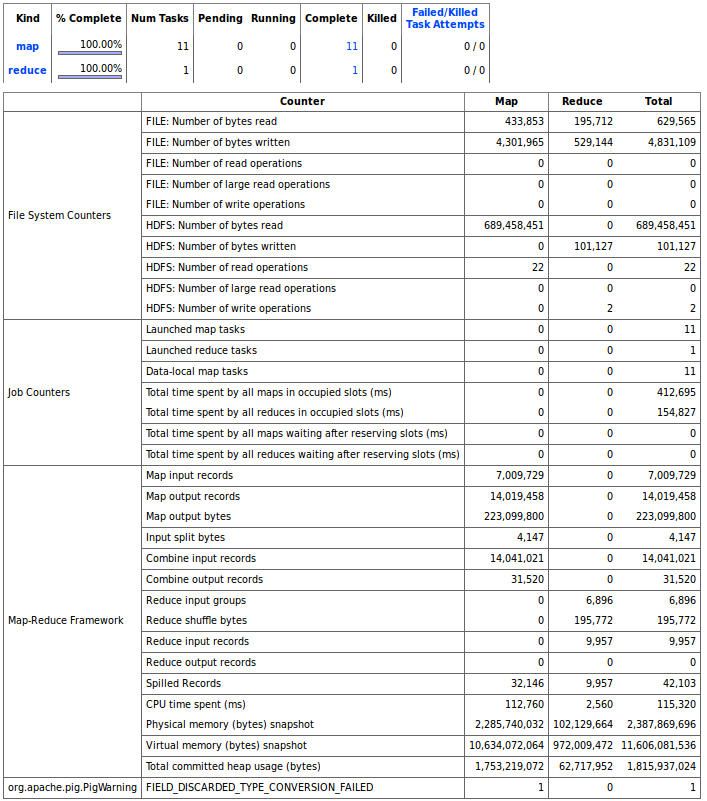
\includegraphics[scale=0.8]{pig1.png}
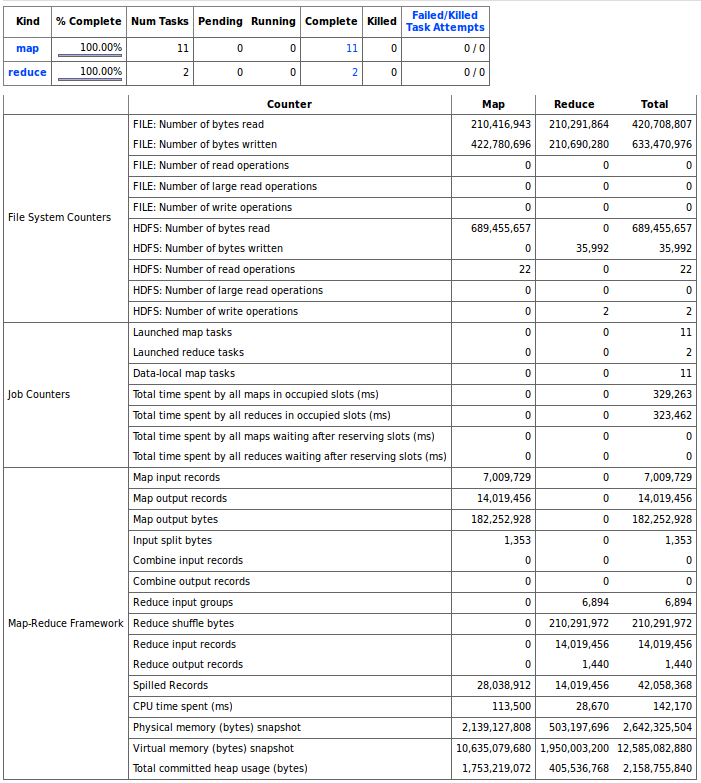
\includegraphics[scale=0.8]{java1.png}

\subsection{Query 2}
Pig: 3 minuti	 Started at: Fri Jun 03 15:18:35 PDT 2016	 Finished at: Fri Jun 03 15:21:07 PDT 2016

Java: 2 minuti	 Started at: Fri Jun 03 15:33:06 PDT 2016	 Finished at: Fri Jun 03 15:35:14 PDT 2016

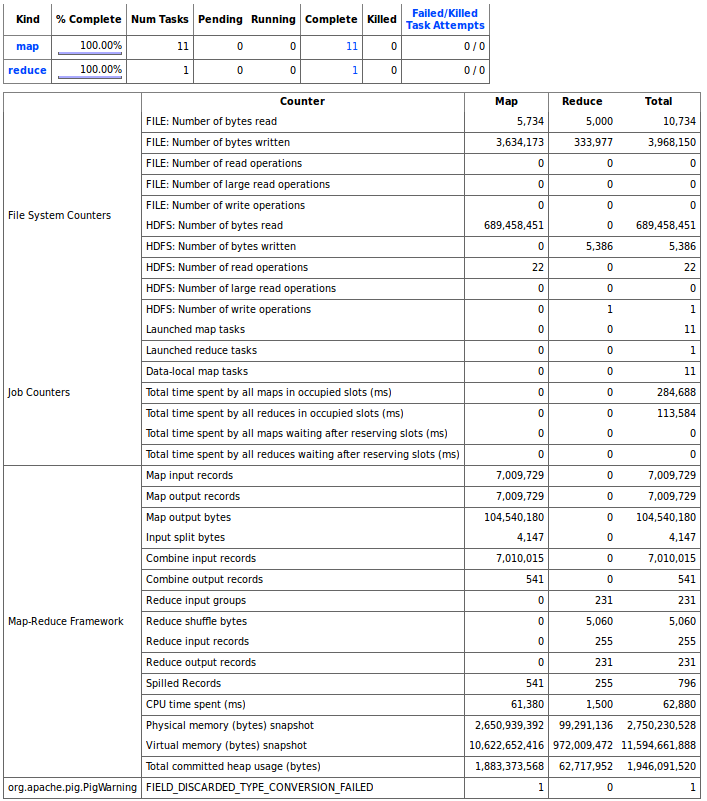
\includegraphics[scale=0.8]{pig2.png}
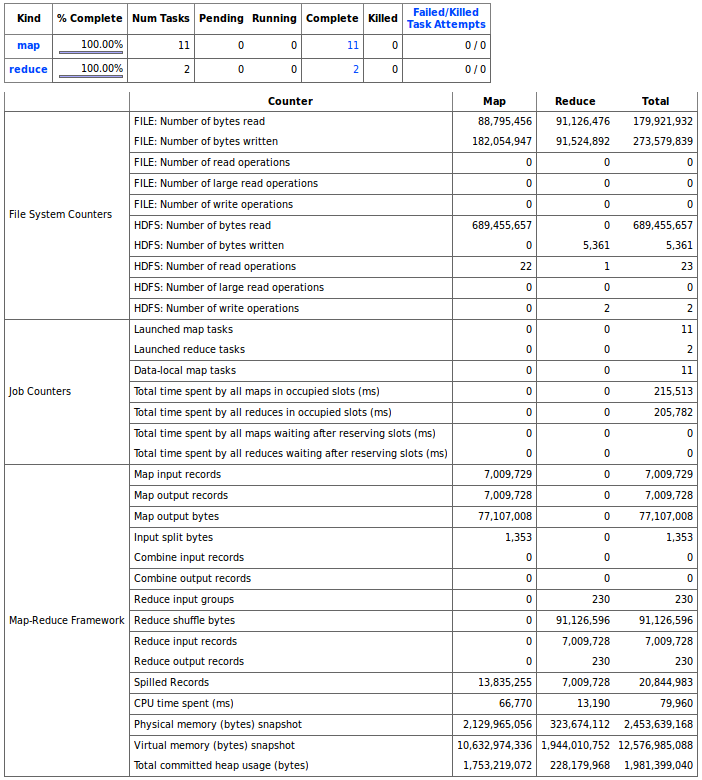
\includegraphics[scale=0.8]{java2.png}

\subsection{Query 3}
Pig: 2 minuti	 Started at: Fri Jun 03 15:38:38 PDT 2016	 Finished at: Fri Jun 03 15:40:41 PDT 2016

Java: 2 minuti	 Started at: Fri Jun 03 15:44:27 PDT 2016	 Finished at: Fri Jun 03 15:46:46 PDT 2016

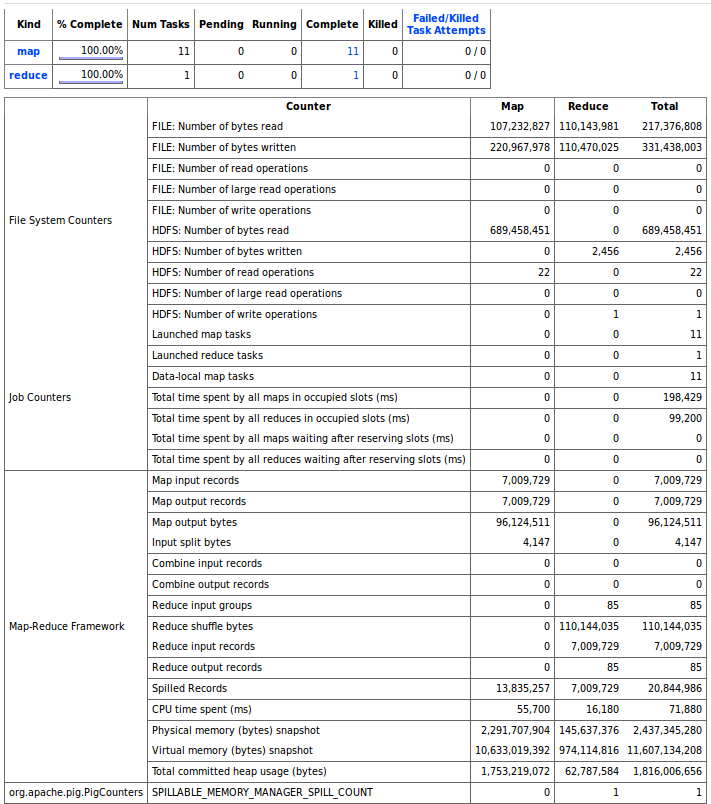
\includegraphics[scale=0.8]{pig3.png}

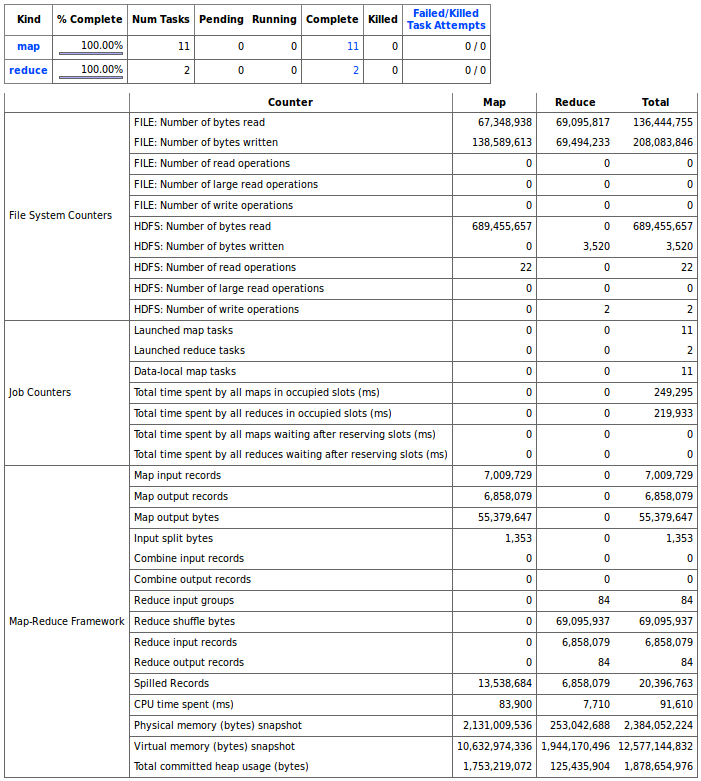
\includegraphics[scale=0.8]{java3.png}

\subsection{Query 4}
Pig: 2 minuti	 Started at: Sat Jun 04 08:27:58 PDT 2016	 Finished at: Sat Jun 04 08:30:05 PDT 2016

Java: 2 minuti	 Started at: Sat Jun 04 08:32:29 PDT 2016	 Finished at: Sat Jun 04 08:35:14 PDT 2016

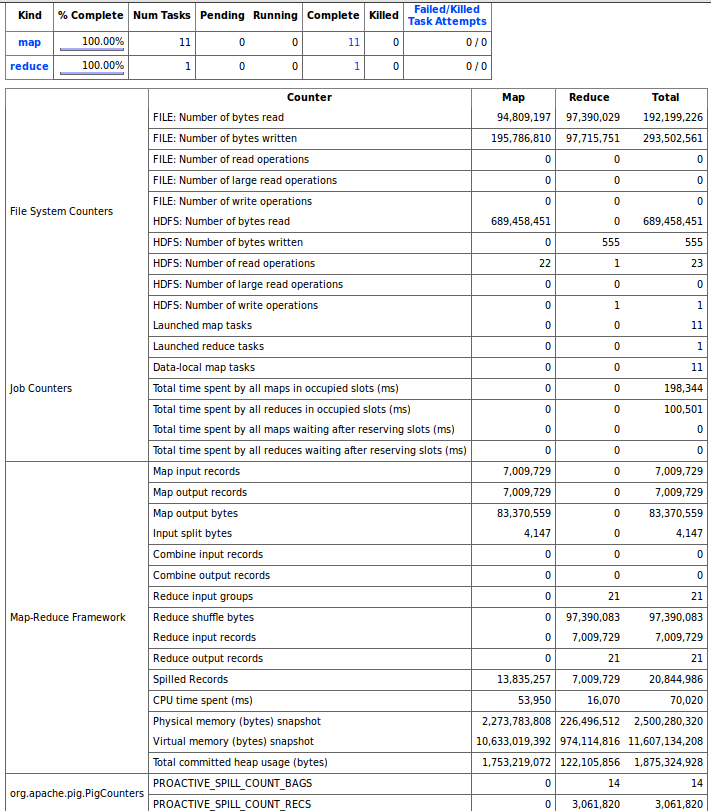
\includegraphics[scale=0.8]{pig4.png}

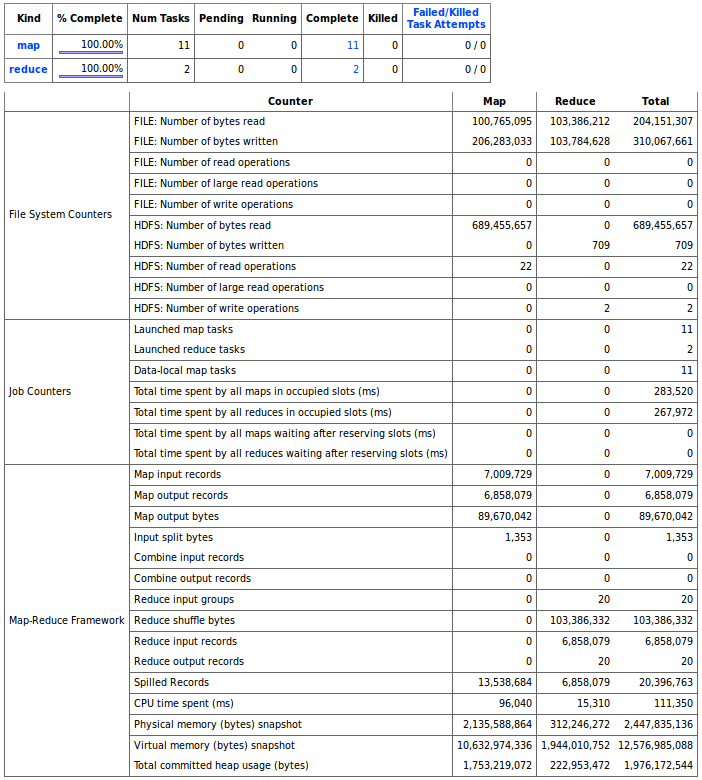
\includegraphics[scale=0.8]{java4.png}

\subsection{Query 5}
Pig:  2 minuti	Started at: Sat Jun 04 08:41:52 PDT 2016	 Finished at: Sat Jun 04 08:44:08 PDT 2016

Java: 3 minuti	Started at: Sat Jun 04 08:53:57 PDT 2016	 Finished at: Sat Jun 04 08:56:57 PDT 2016

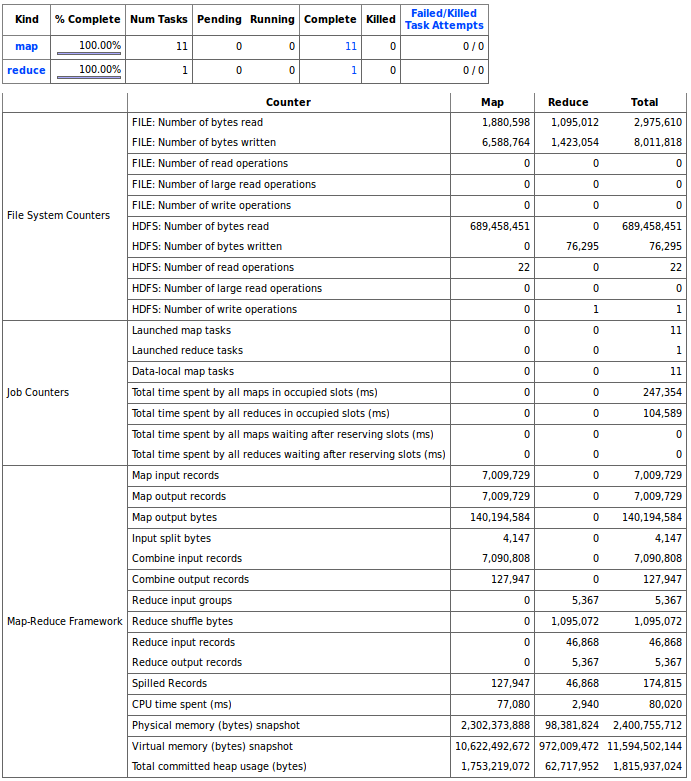
\includegraphics[scale=0.8]{pig5.png}
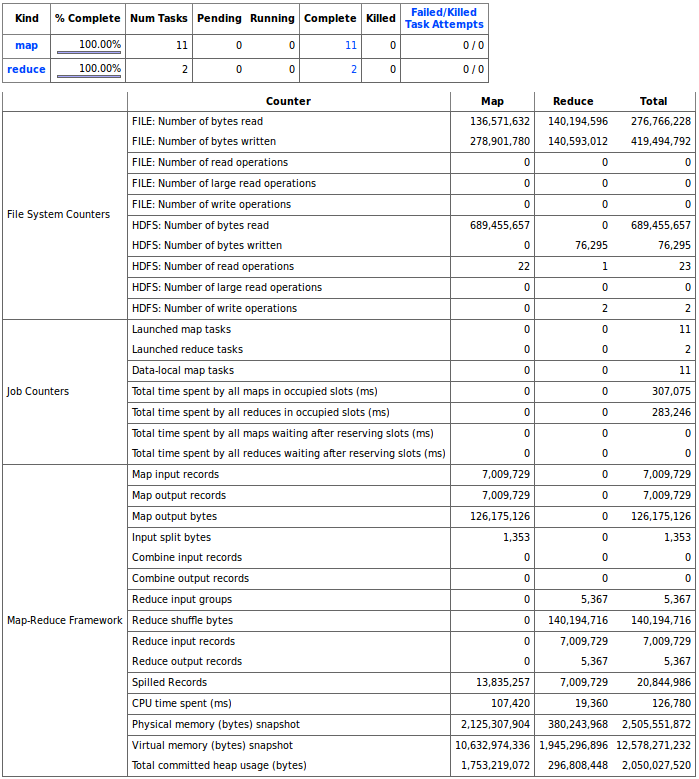
\includegraphics[scale=0.8]{java5.png}

\section{Osservazioni personali}

Una differenza sostanziale tra i due sistemi si nota sui tempi di sviluppo. Per le query in Pig, ci sono volute poche ore per implementare le 5 query (circa 12 ore) e poco tempo per testare il tutto; questo perché Pig è stato concepito per sviluppare velocemente calcolo distribuito. Per la parte in Java MapReduce invece, ci sono voluti molti giorni (circa 6 giorni), soprattutto per la prima query in quanto era necessario adottare dei meccanismi non banali, oltre a delle competenze avanzate sulla conoscenza e ridefinizione del sistema. Quindi, dal punto di vista delle tempistiche di progettazione, risulta migliore Pig.

~

Il codice inoltre risulta molto più leggibile il codice di Pig, in quanto è molto comprensibile (anche nella scelta dei nomi delle funzioni) e più ordinato, poiché si scrive solo il procedimento da eseguire per effettuare una query; in Java MapReduce invece risulta meno leggibile in quanto è presente molto più codice e si devono definire, oltre alla procedura delle query, il codice che configura tutto il sistema.

~

\'E stata più facile anche la soluzione di bug in Pig, in quanto è molto più chiaro il codice e quindi più facili da debuggare.

~

Infine, la progettazione è più facile in Pig in quanto la progettazione è più intuitiva, non necessita di particolari competenze e non bisogna ragionare come fosse un codice parallelo, ma come fosse codice MySQL. Invece in Java MapReduce bisogna ragionare in modo diverso, in quanto è necessario capire come si comportano Mapper e Reducer e quali tipi di dati devono inviarsi.

~

A favore di Java MapReduce invece si può parlare di maggiore controllo sia di progettazione sia di efficienza, in quanto è possibile definire filtri e regole di query molto più precise rispetto a Pig, soprattutto per il controllo del codice. Sviluppando infatti in Java, si possono sfruttare le capacità di programmazione di quest'ultimo per creare codice molto più efficiente, che per queste query non si nota per la durata computazionale, ma si nota sul risultato di output, che risulta molto più preciso di Pig. Pig esegue infatti una semplice analisi di ogni riga per estrapolare il contenuto interessato, invece con Java si riesce a lavorare molto più facilmente con ogni campo delle entry trattandole come stringhe e poi come oggetti nel caso delle chiavi composte.

~

Pig inoltre dovrebbe rendere più performante il codice in maniera automatica utilizzando un'analisi semantica del codice, in modo da concentrarsi sul risultato finale e non sul modo in cui ottenerlo, però per query complesse è molto più utile ragionare sul metodo con cui si ottengono i risultati, poichè il risultato può sempre essere raffinato in un secondo momento.

~
 
Per sopperire ad alcune mancanze di Pig, si possono comunque usare le UDF (User Defined Functions) o programmi esterni, che vanno incontro a tutti i problemi progettuali che si possono riscontrare in Pig, però è buona norma non abusarne, poichè questo sistema esegue ottimizzazioni sul codice scritto nel suo linguaggio, ma non su programmi importati esternamente, quindi si possono creare problemi di spreco di risorse e quindi si può peggiorare o addirittura perdere l'efficienza di Pig.

~

Un altro problema che differenzia Pig da Java MapReduce è la compilazione e le dipendenze: Pig risulta molto più portabile e mantenibile in questo senso rispetto a Java MapReduce in quanto non necessita di compilazione o di una versione particolare che necessita di soddisfacimento di dipendenze, al contrario di Java. Per sviluppare in Java MapReduce bisogna mantenere l'ambiente di compilazione sempre aggiornato, anche per utilizzare nuove forme di programmazione che possono migliorare la programmazione e velocizzare il codice, senza ricompilare tutto e generare nuovamente il file Jar.



\end{document}
